%Version 3 December 2023
% See section 11 of the User Manual for version history
%
%%%%%%%%%%%%%%%%%%%%%%%%%%%%%%%%%%%%%%%%%%%%%%%%%%%%%%%%%%%%%%%%%%%%%%
%%                                                                 %%
%% Please do not use \input{...} to include other tex files.       %%
%% Submit your LaTeX manuscript as one .tex document.              %%
%%                                                                 %%
%% All additional figures and files should be attached             %%
%% separately and not embedded in the \TeX\ document itself.       %%
%%                                                                 %%
%%%%%%%%%%%%%%%%%%%%%%%%%%%%%%%%%%%%%%%%%%%%%%%%%%%%%%%%%%%%%%%%%%%%%

%%\documentclass[referee,sn-basic]{sn-jnl}% referee option is meant for double line spacing

%%=======================================================%%
%% to print line numbers in the margin use lineno option %%
%%=======================================================%%

%%\documentclass[lineno,sn-basic]{sn-jnl}% Basic Springer Nature Reference Style/Chemistry Reference Style

%%======================================================%%
%% to compile with pdflatex/xelatex use pdflatex option %%
%%======================================================%%

%%\documentclass[pdflatex,sn-basic]{sn-jnl}% Basic Springer Nature Reference Style/Chemistry Reference Style


%%Note: the following reference styles support Namedate and Numbered referencing. By default the style follows the most common style. To switch between the options you can add or remove “Numbered” in the optional parenthesis. 
%%The option is available for: sn-basic.bst, sn-vancouver.bst, sn-chicago.bst%  
 
%%\documentclass[pdflatex,sn-nature]{sn-jnl}% Style for submissions to Nature Portfolio journals
%%\documentclass[pdflatex,sn-basic]{sn-jnl}% Basic Springer Nature Reference Style/Chemistry Reference Style
\documentclass[pdflatex,sn-mathphys-num]{sn-jnl}% Math and Physical Sciences Numbered Reference Style 
%%\documentclass[pdflatex,sn-mathphys-ay]{sn-jnl}% Math and Physical Sciences Author Year Reference Style
%%\documentclass[pdflatex,sn-aps]{sn-jnl}% American Physical Society (APS) Reference Style
%%\documentclass[pdflatex,sn-vancouver,Numbered]{sn-jnl}% Vancouver Reference Style
%%\documentclass[pdflatex,sn-apa]{sn-jnl}% APA Reference Style 
%%\documentclass[pdflatex,sn-chicago]{sn-jnl}% Chicago-based Humanities Reference Style

%%%% Standard Packages
%%<additional latex packages if required can be included here>

\usepackage{graphicx}%
\usepackage{multirow}%
\usepackage{amsmath,amssymb,amsfonts}%
\usepackage{amsthm}%
\usepackage{mathrsfs}%
\usepackage[title]{appendix}%
\usepackage{xcolor}%
\usepackage{color, colortbl}
\usepackage{textcomp}%
\usepackage{manyfoot}%
\usepackage{booktabs}%
\usepackage{algorithm}%
\usepackage{algorithmicx}%
\usepackage{algpseudocode}%
\usepackage{listings}%
\usepackage{comment}
%%%%


%% as per the requirement new theorem styles can be included as shown below
\theoremstyle{thmstyleone}%
\newtheorem{theorem}{Theorem}%  meant for continuous numbers
%%\newtheorem{theorem}{Theorem}[section]% meant for sectionwise numbers
%% optional argument [theorem] produces theorem numbering sequence instead of independent numbers for Proposition
\newtheorem{proposition}[theorem]{Proposition}% 
%%\newtheorem{proposition}{Proposition}% to get separate numbers for theorem and proposition etc.

\theoremstyle{thmstyletwo}%
\newtheorem{example}{Example}%
\newtheorem{remark}{Remark}%

\theoremstyle{thmstylethree}%
\newtheorem{definition}{Definition}%

\raggedbottom
%%\unnumbered% uncomment this for unnumbered level heads

\begin{document}

\title[Article Title]{Bayesian Evidence of alternative models of P2X2 activation}

\author*[1]{\fnm{Luciano} \sur{Moffatt}}\email{lmoffatt@qi.fcen.uba.ar}
\author[2]{\fnm{Gustavo} \sur{Pierdominici-Sottile}}\email{gsottile@unq.edu.ar}
%\equalcont{These authors contributed equally to this work.}

%\author[1,2]{\fnm{Third} \sur{Author}}\email{iiiauthor@gmail.com}
%\equalcont{These authors contributed equally to this work.}

\affil*[1]{\orgdiv{Instituto de Qu\'{i}mica F\'{i}sica de los Materiales, Medio Ambiente y Energ\'{i}a}, \orgname{  Consejo Nacional de Investigaciones Científicas y T\'{e}cnicas}, \orgname{Universidad de Buenos Aires} , \city{Buenos Aires}, \postcode{1428},  \country{Argentina}}

\affil[2]{\orgdiv{Departamento de Ciencia y Tecnolog\'{i}a, 
  Consejo Nacional de Investigaciones Científicas y T\'{e}cnicas} \orgname{Universidad Nacional de Quilmes}, \orgaddress{\street{S\'{a}enz Pe\~{n}a 352}, \city{Bernal}, \postcode{B1876BXD}, \state{Buenos Aires}, \country{Argentina}}}

%\affil[3]{\orgdiv{Department}, \orgname{Organization}, \orgaddress{\street{Street}, \city{City}, \postcode{610101}, \state{State}, \country{Country}}}

\begin{comment}
ESTAMOS 78 PALABRAS ENCIMA DE LO SUGERIDO
\end{comment}


\abstract{Ligand-activated receptors are essential for cellular signaling and represent significant therapeutic targets. Among these, the P2X receptor family, activated by ATP, plays a crucial role in various physiological processes, yet the molecular mechanisms governing its activation remain inadequately understood, particularly regarding the conformational dynamics between subunit interactions. Here, we demonstrate that ATP binding induces asymmetric conformational changes in the P2X receptor, specifically driving the rotation of the subunit bound by the upper body (UB), while the lower body (LB)-bound subunit remains stationary. We re-analyze previously published data from outside-out patch preparations of rP2X2 in response to ultra-short ATP pulses of varying concentrations (0.2-10 mM) using a novel Bayesian algorithm that leverages kinetic information from response fluctuations. This analysis reveals that agonist binding promotes rotational shifts in the UB subunit 100 to 10,000 times more  than in the LB subunit. UB subunit rotation accelerates agonist binding and delays release, whereas LB subunit rotation slows both processes. Our findings elucidate distinct roles at the subunit interfaces: the UP subunit functions as an anchor, while LB subunit rotation enhances ATP binding energy and stabilizes the receptor in its active state. Once rotated, the UP subunit shields ATP, limiting its exchangeability and further stabilizing the binding site.

We anticipate that our Bayesian kinetic analysis will be instrumental in validating and refining the activation model presented here. This framework can be extended to investigate mutations, partial agonists, and other subunits. Furthermore, the notion of one subunit acting as an anchor while another serves as an allosterically active component may be applicable to other ligand-activated receptors. These insights could pave the way for developing innovative pharmaceutical agents targeting P2X receptors and related signaling pathways.
}




%%================================%%
%% Sample for structured abstract %%
%%================================%%

% \abstract{\textbf{Purpose:} As a guide the abstract should not exceed 200 words. Most journals do not set a hard limit however authors are advised to check the author instructions for the journal they are submitting to.
% 
% \textbf{Methods:} The abstract serves both as a general introduction to the topic and as a brief, non-technical summary of the main results and their implications. The abstract must not include subheadings (unless expressly permitted in the journal's Instructions to Authors), equations or citations. As a guide the abstract should not exceed 200 words. Most journals do not set a hard limit however authors are advised to check the author instructions for the journal they are submitting to.
% 
% \textbf{Results:} The abstract serves both as a general introduction to the topic and as a brief, non-technical summary of the main results and their implications. The abstract must not include subheadings (unless expressly permitted in the journal's Instructions to Authors), equations or citations. As a guide the abstract should not exceed 200 words. Most journals do not set a hard limit however authors are advised to check the author instructions for the journal they are submitting to.
% 
% \textbf{Conclusion:} The abstract serves both as a general introduction to the topic and as a brief, non-technical summary of the main results and their implications. The abstract must not include subheadings (unless expressly permitted in the journal's Instructions to Authors), equations or citations. As a guide the abstract should not exceed 200 words. Most journals do not set a hard limit however authors are advised to check the author instructions for the journal they are submitting to.}

\keywords{Bayesian Analysis, P2X receptors, Cellular Signaling}

\maketitle

\section{Introduction}
\label{sec1}


Ligand-gated ion channels (LGICs) are multimeric membrane proteins that allow ions to cross the cell membrane in response to ligand binding \cite{p2x_cuerpo_humano}. These channels play critical roles in synaptic transmission, muscle contraction, and other physiological processes (add them), making them important targets in neuropharmacology \cite{p2x_drugs,therapeutic,p2x7_pharmacology}. LGIC families are classified based on their subunit composition and the location of ligand-binding sites. In pentameric Cys-loop receptors, the binding site is located at the interface between adjacent subunits, while in tetrameric glutamate receptors, it is within individual subunits. In trimeric P2X receptors, like Cys-loop receptors, the binding sites are located between subunits.

P2X receptors are the only LGICs for which high-resolution structures of both open and closed conformations are available \cite{cerrada_p2x,abierta_p2x}. These structures reveal that ATP binding triggers a rotational movement in all three subunits, leading to the separation of the transmembrane domains that form the pore, allowing ions to pass through. However, the intermediate states between these conformations remain unresolved. Understanding these intermediate states is essential for elucidating the mechanism of channel opening, which could inform the design of drugs that modulate P2X receptor function.

Two types of gating models have been proposed for P2X receptor activation: sequential rotation models, where subunits rotate one at a time to gradually open the pore, and synchronous models, where all subunits rotate together in a concerted motion. In sequential models, a key question arises about potential asymmetry: whether one subunit rotates first, specifically the subunit bound to the ATP by the Upper Body (UB) or the one bound by the Lower Body (LB). Addressing this question is essential for comprehending the complete activation mechanism of P2X receptors, which could pave the way for innovative pharmacological designs.. 

In the case of P2X2 receptors, recordings of macroscopic currents in response to ultrashort (0.2 ms) ATP pulses provide valuable insights into the channel's activation process \cite{Moffatt_hume}. Previous models fitted to these data have proposed both sequential and synchronous gating schemes. However, early models incorrectly assumed intrasubunit binding sites akin to glutamate receptors, and no direct comparison of the evidence for the two gating models has been performed. 

Macrocurrents reflect the collective activity of numerous channels. The fluctuations in these currents contain valuable kinetic information. To analyze these fluctuations, we developed a novel algorithm, MacroIR, which improves the Macroscopic Recursive (MacroR) algorithm by accounting for finite integration times in voltage clamp recordings. MacroIR calculates the mean conductance and its variance over specified time intervals, providing a more accurate approximation of the likelihood function.

In this study, we applied MacroIR to our previously published recordings of ultrashort ATP pulses to investigate P2X2 receptor gating. We introduced new sequential gating schemes that take into account the inter-subunit binding sites and implement an affine-invariant Monte Carlo Markov chain (MCMC) algorithm to calculate posterior distributions and model evidence. Our results reveal that a sequential model with asymmetric allosteric coupling has a stronger evidence than either symmetric sequential or synchronous models. Our study provides a novel framework for analyzing gating mechanisms in P2X2 receptors by combining advanced kinetic modeling with the MacroIR algorithm, offering new insights into receptor activation.

\section{Methods}
\label{sec:methods}

\subsection{Notation}
We denote specific channel states using subscripts (e.g., \( i, j \)), while superscripts (e.g., "prior", "post", "obs") are used to indicate the type of probability distribution (e.g., prior, posterior, or observed). For instance, \( p_i^{\text{prior}} \) represents the prior probability of being in state \( i \), and \( p_i^{\text{post}} \) represents the posterior probability after an observation.

\subsection{Markov model of single-channel behavior}

Early studies of single-channel recordings revealed that ion channels exhibit stochastic opening and closing at irregular intervals, consistent with the thermal fluctuations that macromolecules experience. Given this stochastic behavior, it is natural to model channel kinetics using a Markov process with a finite set of states \( k \), where each state represents a subset of the channel protein’s conformational landscape. 

A Markov process does not specify the precise conformation of the channel at any given moment; instead, it yields the probability vector \( \boldsymbol{p} \), where each element \( p_i \) represents the likelihood of the channel being in state \( i \). The model assumes a constant transition rate, \( k_{ij} \), for jumps between states \( i \) and \( j \). The time evolution of the probability vector \( \boldsymbol{p}(t) \) is governed by the following first-order differential equation:

\begin{equation}
	\frac{d \boldsymbol{p}}{dt}(t) = \boldsymbol{p}(t) \cdot \boldsymbol{Q}(t),
	\label{eq:master_equation}
\end{equation}

where the off-diagonal elements of the matrix \( \boldsymbol{Q} \) are given by the transition rates \( k_{ij} \). The diagonal elements \( k_{ii} \) are defined to ensure probability conservation:

\begin{align}
	k_{ii} = -\sum_{j, j \neq i} k_{ij}.
	\label{eq:Q_diagonal_element}
\end{align}

This formulation ensures that the total probability remains normalized over time, with the transitions between states governed by the rates encoded in the matrix \( \boldsymbol{Q} \). The Markovian framework thus reduces the complex conformational dynamics of the channel into a tractable probabilistic model, allowing for detailed analysis of the channel gating kinetics.


The integration of Eq.~\ref{eq:master_equation} allows us to determine the time evolution of the probability vector \( \boldsymbol{p}(t) \). This integration yields:


\begin{align}
	\boldsymbol{p}(t) &= \boldsymbol{p}(0) \cdot \boldsymbol{P}(t)
	\label{eq:master_equation_solution}
\end{align}
\begin{align}
	\boldsymbol{P} (t) &= \exp(\boldsymbol{Q} \cdot t),
	\label{eq:Transition_Matrix_definition}
\end{align}


where \( \exp(\boldsymbol{Q} \cdot t) \) is the matrix exponential of \( \boldsymbol{Q} \) multiplied by time \( t \). 

In this context, the actual state of the Markov process remains unobservable; what can be directly measured is the current produced by the channel. Each state \( i \) of the channel generates a specific single-channel current, encoded in the current vector \( \boldsymbol{\gamma} \). The observable current at any given time is thus determined by the probability-weighted sum over all states, which can be expressed as:

\begin{equation}
	y^{\text{pred}}(t) = \boldsymbol{p}(t) \cdot \boldsymbol{\gamma}.
	\label{eq:single_channel_prediction}
\end{equation}

This relationship links the hidden Markov states to the measurable macroscopic current, allowing us to infer the channel kinetics from experimental recordings.



\subsection{MicroR, Bayesian model for instantaneous measurements of single-channel behavior}

The microscopic recursive term was coined for the exact description of an ensemble of channels, however the equations are the same that for single channels, so we extend the term to cover the classical bayesian analysis fo single channels. 
Consider the scenario where we perform a single "instantaneous" current measurement, denoted as \( y^{\text{obs}} \). Let the initial state probability distribution be given by \( \boldsymbol{p}^{\text{prior}} \). Suppose the instrumental noise associated with each measurement follows a normal distribution with variance \( \epsilon^2 \). Under these conditions, we can derive the likelihood of the measurement and update the posterior probability distribution accordingly.

Using the state current $\gamma_i$, the likelihood of observing the current \( y^{\text{obs}} \) is given by:

\begin{equation}
	\mathcal{L} = P(y^{\text{obs}}) = \sum_i \mathcal{N}(p_i \cdot \gamma_i, \epsilon^2),
	\label{eq:single_channel_likelihood}
\end{equation}

where \( \mathcal{N}(\mu, \sigma^2) \) denotes the normal distribution with mean \( \mu \) and variance \( \sigma^2 \).

The posterior probability distribution, \( \boldsymbol{p}^{\text{post}} \), is then updated using Bayes' rule:

\begin{equation}
	p^{\text{post}}_i = p_i \cdot \frac{\mathcal{N}(p_i \cdot \gamma_i, \epsilon^2)}{P(y^{\text{obs}})},
	\label{eq:single_channel_posterior}
\end{equation}

where \( p^{\text{post}}_i \) denotes the posterior probability of state \( i \) after observing the measurement.

Now, suppose a second measurement is taken after a time interval \( t \). The prior probability distribution at time \( t \), denoted \( \boldsymbol{p}^{\text{prior}}(t) \), is obtained by applying Eq.~\ref{eq:master_equation_solution}:

\begin{align}
	\boldsymbol{p}^{\text{prior}}(t) &= \boldsymbol{p}^{\text{post}}(0) \cdot \boldsymbol{P}(t)
	\label{eq:prior_update}
\end{align}

where \( \boldsymbol{Q} \) is the rate matrix governing the Markov process.

Since the probability of each observation \( {y}_n^{\text{obs}} \) is calculated conditionally on the previous observations \( {y}_1^{\text{obs}}, \dots, {y}_{n-1}^{\text{obs}} \), the cumulative log-likelihood of the entire measurement series can be obtained:

\begin{equation}
	\log \mathcal{L} = \sum_i \log (\mathcal{L}_i),
	\label{eq:total_loglikelihood}
\end{equation}

where \( \mathcal{L}_i \) corresponds to the likelihood of the \( i \)-th measurement.


\subsection{MicroIR, the Bayesian Model of Time-Averaged Single-Channel Measurements}

This new algorithm allows to analyze hidden markovian processes where the information we gain from them results from a time-weighed averaged response,as opposed as from an instantaneous observation. It is another solution for the missing events problem, but from a different perspective, one that does not intend to idealize the recording but to directly calculate the likelihood. This would allow to compare the evidence of alternative kinetic models, something that is not straightforward when an idealization step is included.  
We did not actually used this algorithm in this paper, it was necessary conceptual step to present MacroIR. We present it for single channels, but a similar argument can be extended for other single molecule systems, where time averaging is even more compelling (like molecular motors). 
We consider a scenario where, instead of instantaneous measurements, we observe the time-averaged current \( \overline{y_t}^{\text{obs}} \) over a specific interval \( t \). During this time interval, the channel state fluctuates continuously, with each specific trajectory representing a point in an infinite-dimensional space—an unwieldy realm for statistical analysis. However, from a Bayesian perspective, there is only one crucial piece of information: the prior probability distribution at the beginning of each interval. The state probabilities at all subsequent times within the interval can be computed using Eq.~\ref{eq:master_equation_solution}. 

On the other hand, there is only one piece of information that we gain from the interval: the observed average current. Ideally, we would like to obtain the posterior probability at the end of the interval so that it can be used as the prior for the next interval. To correctly compute this posterior distribution, we must account for both the starting and ending states.

Given the prior state probability distribution \( \boldsymbol{p}^{\text{prior}} \) at the start of the interval, we can calculate the joint state probability matrix \( \boldsymbol{\Pi} \), where the elements \( \Pi_{i \rightarrow j} \) represent the probability of starting in state \( i \) and ending in state \( j \):

\begin{equation}
	\Pi_{i \rightarrow j}^{\text{prior}} = p^{\text{prior}}_i \cdot P_{i \rightarrow j}
	\label{eq:joint_state_probability}
\end{equation}

Here, \( P_{i \rightarrow j} \) denotes the probability of transitioning from state \( i \) to state \( j \).

Alternatively, in matrix form:

\begin{equation}
	\boldsymbol{\Pi}^{\text{prior}} = \mathrm{diag}(\boldsymbol{p}^{\text{prior}}) \cdot \mathbf{P}
	\label{eq:joint_state_probability_matrix}
\end{equation}

The probability of an observed average current \( \overline{y}^{\text{obs}} \) result form Eq.~\ref{eq:single_channel_likelihood}:

\begin{equation}
	\mathcal{L}=P(\overline{y}^{\text{obs}}) = \sum_{i, j} \Pi_{i \rightarrow j}^{\text{prior}} \cdot \mathcal{N}\left(\overline{y}^{\text{obs}} - \Pi_{i \rightarrow j}^{\text{prior}} \cdot \overline{\Gamma}_{i \rightarrow j}, \epsilon^2 + \sigma^2_{\overline{\Gamma}_{i \rightarrow j}}\right)
	\label{eq:single_channel_integrated_likelihood}
\end{equation}

where \( \overline{\Gamma}_{i \rightarrow j} \) and \( \sigma^2_{\overline{\Gamma}_{i \rightarrow j}} \) represent the average current and its variance for trajectories starting in state \( i \) and ending in state \( j \), respectively.

The posterior distribution of the joint state probability matrix is updated using Bayes' theorem:

\begin{equation}
	\Pi_{i \rightarrow j}^{\text{post}} = \frac{\Pi_{i \rightarrow j}^{\text{prior}} \cdot \mathcal{N}\left(\overline{y}^{\text{obs}} - \Pi_{i \rightarrow j}^{\text{prior}} \cdot \overline{\Gamma}_{i \rightarrow j}, \epsilon^2 + \sigma^2_{\overline{\Gamma}_{i \rightarrow j}}\right)}{P(\overline{y}^{\text{obs}})}
	\label{eq:single_channel_integrated_posterior}
\end{equation}

The prior state probability distribution for the next interval is then obtained by marginalizing over the initial state \( i \):

\begin{equation}
	p_j^{\text{prior}}(t_{n+1}) = \sum_i \Pi_{i \rightarrow j}^{\text{post}}(t_n)
	\label{eq:single_channel_integrated_next_prior}
\end{equation}

Since the probability of each observation \( \overline{y}_n^{\text{obs}} \) is calculated conditionally on the previous observations \( \overline{y}_1^{\text{obs}}, \dots, \overline{y}_{n-1}^{\text{obs}} \), the cumulative log-likelihood of the entire measurement series can be updated using Eq. \ref{eq:total_loglikelihood}:

\begin{equation}
	\log \mathcal{L}(\overline{y}_1^{\text{obs}}, \dots, \overline{y}_{n+1}^{\text{obs}}) = \log \mathcal{L}(\overline{y}_1^{\text{obs}}, \dots, \overline{y}_n^{\text{obs}}) + \log P(\overline{y}_{n+1}^{\text{obs}})
	\label{eq:single_channel_integrated_total_likelihood}
\end{equation}

While the exact distribution of the mean current is not strictly normal, we approximate it as such, assuming that instrumental noise dominates over gating noise.

\subsubsection{Calculation of the Average Current Conditional on Starting and Ending States}

We calculate the average current \( \overline{\Gamma}_{i \rightarrow j} \) and its variance \( \sigma^2_{\overline{\Gamma}_{i \rightarrow j}} \) for transitions from state \( i \) to state \( j \) during a measurement interval \( t \).

The average current \( \overline{\Gamma}_{i \rightarrow j} \) is computed as the time-weighted average of the current in each state, weighted by the probability of being in that state during the interval:

\begin{equation}
	\overline{\Gamma}_{i \rightarrow j} = \frac{1}{t \cdot P_{i \rightarrow j}} \int_0^t \sum_k P_{i \rightarrow k}(\tau) \, \gamma_k \, P_{k \rightarrow j}(t - \tau) \, d\tau
	\label{eq:gamma_ij_integral}
\end{equation}

Here, \( P_{i \rightarrow j} \) is the probability of transitioning from state \( i \) to state \( j \) within time \( t \), \( P_{i \rightarrow k}(\tau) \) denotes the probability of transitioning from state \( i \) to state \( k \) at time \( \tau \), and \( \gamma_k \) is the current associated with state \( k \).

To efficiently evaluate this integral, we use a spectral form of the matrix exponential, yielding a closed-form expression:

\begin{equation}
	\overline{\Gamma}_{i \rightarrow j} = \frac{1}{P_{i \rightarrow j}} \sum_{k, n_1, n_2} V_{i n_1} \cdot V^{-1}_{n_1 k} \cdot \gamma_k \cdot V_{k n_2} \cdot V^{-1}_{n_2 j} \cdot E_2(\lambda_{n_1} \cdot t, \lambda_{n_2} \cdot t)
	\label{eq:gamma_ij_formula}
\end{equation}

where:
- \( \mathbf{V} \) and \( \mathbf{V}^{-1} \) are the matrices of eigenvectors of the rate matrix \( \mathbf{Q} \) and its inverse, respectively.
- \( \boldsymbol{\lambda} \) is the vector of eigenvalues of \( \mathbf{Q} \).
- The function \( E_2(x, y) \) is defined as:

\begin{equation}
	E_2(x, y) = 
	\begin{cases}
		\frac{\exp(x) - \exp(y)}{x - y}, & \text{if } x \neq y \\
		\exp(x), & \text{if } x = y
	\end{cases}
    \label{eq:E_2}
\end{equation}


\subsubsection{Calculation of the Variance of the Average Current Conditional on Starting and Ending States}

The variance of the average current, conditional on starting in state \(i\) and ending in state \(j\), is defined as the difference between the expected square of the average current and the square of the expected current:

\begin{equation}
	\sigma^2 \overline{\Gamma}_{i \rightarrow j}=\text{Var}(\overline{\Gamma}_{i \rightarrow j}) = E(\overline{\Gamma}_{i \rightarrow j}^2) - P_{i \rightarrow j} \cdot \left( E(\overline{\Gamma}_{i \rightarrow j}) \right)^2
    \label{eq:sigma_gamma_expression}
\end{equation}

where \( E(\overline{\Gamma}_{i \rightarrow j}^2) \) is the expected square of the average current, and \( E(\overline{\Gamma}_{i \rightarrow j}) \) is the expected average current.


To calculate the expected square of the average current, we consider the time-weighted average of the product of the currents at each pair of time points within the interval. This involves summing over all possible intermediate states \(k_1\) and \(k_2\) for the first and second currents, respectively. Specifically, we integrate over the full time interval, accounting for all combinations of transition probabilities at each time point:

\begin{equation}
	E(\overline{\Gamma}_{i \rightarrow j}^2) = \frac{1}{t^2 P_{i \rightarrow j}} \int_0^t \int_0^{t-\tau_1} \sum_{k_1, k_2} P_{i \rightarrow k_1}(\tau_1) \gamma_{k_1} P_{k_1 \rightarrow k_2}(\tau_2) \gamma_{k_2} P_{k_2 \rightarrow j}(t-\tau_1-\tau_2) d\tau_1 d\tau_2
    \label{eq:sqr_gamma_integral}
\end{equation}

Here, \(P_{i \rightarrow k_1}(\tau_1)\) and \(P_{k_1 \rightarrow k_2}(\tau_2)\) represent the transition probabilities between states over the respective time intervals \(\tau_1\) and \(\tau_2\), and \(\gamma_{k_1}\) and \(\gamma_{k_2}\) denote the currents in those states.


By utilizing the spectral decomposition of the transition rate matrix, we can obtain a closed-form expression for the expected square of the average current. This allows us to express the quantity in terms of matrix products and the eigenvalues of the transition rate matrix, as shown below:

\begin{equation}
	E(\overline{\Gamma}_{i \rightarrow j}^2) = \frac{1}{P_{i \rightarrow j}} \sum_{k_1, k_2, n_1, n_2, n_3} V_{i n_1} \cdot V^{-1}_{n_1 k_1} \cdot \gamma_{k_1} \cdot V_{k_1 n_2} \cdot V^{-1}_{n_2 k_2} \cdot \gamma_{k_2} \cdot V_{k_2 n_3} \cdot V^{-1}_{n_3 j} E_3(\lambda_{n_1} \cdot t, \lambda_{n_2} \cdot t, \lambda_{n_3} \cdot t)
    \label{eq:sqr_gamma_formula}
\end{equation}

Here, \(E_3\) is a function that acts on the eigenvalues of the transition rate matrix, and is defined as follows:

\begin{equation}
	E_3(x,y,z)= 
	\begin{cases}
		E_{111}(x,y,z) & x\neq y, y\neq z, z\neq x \\
		E_{12}(x,y) & x\neq y, x\neq z, y = z \\
		E_{12}(y,z) & y\neq z, y\neq x, z = x \\
		E_{12}(z,x) & z\neq x, z\neq y, x = y \\
		\frac{1}{2} \cdot \exp(x) & x=y=z
	\end{cases}
	\label{eq:E_3}
\end{equation}

The function \(E_{12}(x, y)\) is defined as:

\begin{equation}
	E_{12}(x,y) = E_{1,11}(x, y, y) + \frac{\exp(y)}{y - x} \cdot \left(\frac{y - x - 1}{y - x}\right)
	\label{eq:E_12}
\end{equation}

Finally, \(E_{1,11}(x, y, z)\) is given by:

\begin{equation}
	E_{1,11}(x, y, z) = \frac{\exp(x)}{(x - y) \cdot (x - z)}
	\label{eq:E_1_11}
\end{equation}

These expressions allow us to compute the expected square of the average current in a system where the transitions between states are governed by a Markov process with a known transition rate matrix.






\subsection{From Single-Channel Analysis to Ensemble Channel Analysis}

When the only information available about an ensemble of ion channels is the state probability vector—which specifies the likelihood of each individual channel being in a particular state—a multinomial distribution describes the probability of observing each possible distinct state count vector. However, once we gain additional information by measuring the total current produced by the ensemble, we can update the posterior distribution of the ensemble state. This updated distribution not only deviates from a multinomial form but also exhibits inverse correlations between states that generate the same current. Although individual channels remain independent, the information we obtain about the ensemble as a whole introduces correlations, reminiscent of quantum entanglement. Thus, we require a method to characterize the posterior probability distribution of the ensemble state that adequately captures these induced correlations.

A precise yet computationally intensive approach involves constructing a vector—referred to as the \textit{ensemble state vector}—that encompasses all possible combinations of state counts and applying Bayes' rule to each entry individually. This method, which I term the \textit{Microscopic Recursive Algorithm}, was detailed in a previous publication (Moffatt, 2007). However, this approach quickly becomes computationally prohibitive as the system size increases.

A more efficient alternative approximates the ensemble state distribution using a multivariate normal distribution of the state count vector. The covariance matrix serves as a first-order approximation to account for the observation-induced correlations between states. This constitutes the \textit{Macroscopic Approach}, significantly simplifying the representation of the ensemble's state distribution.

\subsection{MacroR, Bayesian Framework for Instantaneous Measurements of Channel Ensembles}

In the \textit{MacroR algorithm}, we treat measurements as instantaneous and focus solely on the ensemble's instantaneous state. This framework leverages both the mean probability vector and the covariance matrix of the probability state, capturing the ensemble's key statistical properties at any given moment. The same results can be obtained from a Kalman filter. 

After integrating the multivariate Gaussian, the likelihood of observing an instantaneous current \( y^{\text{obs}} \) can be obtained:

\begin{equation}
	\mathcal{L} = \mathcal{N} \left( y^{\text{obs}} - y^{\text{pred}}, \sigma^2_{y^{\text{pred}}} \right)
	\label{eq:macro_likelihood}
\end{equation}

where \( y^{\text{pred}} \), the prediction of the kinetic model for the subsequent observation, is given by:

\begin{equation}
	y^{\text{pred}} = N_{\text{ch}} \cdot \boldsymbol{\mu}^{\text{prior}} \cdot \boldsymbol{\gamma}
	\label{eq:macro_predicted_y}
\end{equation}

Here, \( \sigma^2_{y^{\text{pred}}} \), the variance of this prediction, which is related to what is usually called gating noise, is:

\begin{equation}
	\sigma^2_{y^{\text{pred}}} = \epsilon^2 + N_{\text{ch}} \cdot \boldsymbol{\gamma}^{\mathrm{T}} \cdot \boldsymbol{\Sigma}^{\text{prior}} \cdot \boldsymbol{\gamma}
	\label{eq:macro_sigma_pred}
\end{equation}

Similarly, we have a closed form for \( \boldsymbol{\mu}^{\text{post}} \), the mean state probability vector, which is the mean of the multivariate Gaussian representing the posterior probability state:

\begin{equation}
	\boldsymbol{\mu}^{\text{post}} = \boldsymbol{\mu}^{\text{prior}} + \frac{y^{\text{obs}} - y^{\text{pred}}}{\sigma^2_{y^{\text{pred}}}} \cdot \boldsymbol{\gamma}^{\mathrm{T}} \cdot \boldsymbol{\Sigma}^{\text{prior}}
	\label{eq:macro_mean_posterior}
\end{equation}

And for \( \boldsymbol{\Sigma}^{\text{post}} \), the covariance of the state probability vector, which represents the covariance of the same multivariate Gaussian:

\begin{equation}
	\boldsymbol{\Sigma}^{\text{post}} = \boldsymbol{\Sigma}^{\text{prior}} - \frac{N}{\sigma^2_{y^{\text{pred}}}} \cdot \boldsymbol{\Sigma}^{\text{prior}} \cdot \boldsymbol{\gamma} \cdot \boldsymbol{\gamma}^{\mathrm{T}} \cdot \boldsymbol{\Sigma}^{\text{prior}}
	\label{eq:macro_cov_posterior}
\end{equation}

Next, we calculate the prior probability at time \( t_{n+1} = t_n + \Delta t_n \) using conditional expectation:

\begin{equation}
	\boldsymbol{\mu}^{\text{prior}}(t_{n+1}) = \boldsymbol{\mu}^{\text{post}}(t_n) \cdot \mathbf{P}(\Delta t_n)
	\label{eq:macro_mean_next_prior}
\end{equation}

And its covariance:

\begin{equation}
	\boldsymbol{\Sigma}^{\text{prior}}(t_{n+1}) = \mathrm{diag}(\boldsymbol{\mu}^{\text{prior}}(t_{n+1})) + \mathbf{P}(\Delta t_n)^{\mathrm{T}} \cdot \left( \boldsymbol{\Sigma}^{\text{post}}(t_n) - \boldsymbol{\mu}^{\text{post}}(t_n) \right) \cdot \mathbf{P}(\Delta t_n)
	\label{eq:macro_mean_next_cov}
\end{equation}

This completes the recursion step of the Macroscopic Recursive algorithm.


\subsection{MacroIR: A Bayesian Framework for Interval-Averaged Analysis of Channel Ensembles}

We introduce MacroIR (Macroscopic Interval Recursive), a novel Bayesian framework designed for time-averaged Markovian processes over successive intervals. The algorithm is inspired by macropatch recordings, which provide high-fidelity kinetic data with low noise. This approach is versatile, extending to systems such as FRET measurements, molecular motor ensembles, and potentially diffusion analyses.

MacroIR applies the MacroR algorithm to the meta-state described in the MicroIR algorithm, which represents the initial and final states within an interval. Importantly, while the meta-state concept theoretically expands the state space from \( k \) to \( k^2 \), leading to a computational cost scaling from \( k^3 \) to \( k^6 \), algebraic simplifications restore the complexity to \( k^3 \). These simplifications eliminate the need for explicit meta-state calculations, enabling efficient updates of the likelihood and posterior distributions.

The meta-state represents the joint probabilities of starting in state \( i_0 \) and ending in state \( i_t \) over a time interval \( [0, t] \). The prior mean is given by:
\begin{equation}
	(\mu^{\text{prior}}_{0 \rightarrow t})_{(i_0 \rightarrow i_t)} = (\mu^{\text{prior}})_{i_0} \cdot P_{i_0 \rightarrow i_t}(t),
	\label{eq:meta_mean_prior}
\end{equation}
where \( P_{i_0 \rightarrow i_t}(t) \) is the transition probability.

Similarly, the prior covariance is:
\begin{multline}
	(\Sigma^{\text{prior}}_{0 \rightarrow t})_{(i_0 \rightarrow i_t)(j_0 \rightarrow j_t)} = 
	P_{i_0 \rightarrow i_t} \big[(\Sigma^{\text{prior}}_0)_{i_0, j_0} - \delta_{i_0, j_0} \cdot (\mu^{\text{prior}}_0)_{i_0} \big] \cdot P_{j_0 \rightarrow j_t} \\
	+ \delta_{i_0, j_0} \cdot \delta_{i_t, j_t} \cdot (\mu^{\text{prior}}_0)_{i_0} \cdot P_{i_0 \rightarrow i_t},
	\label{eq:meta_covariance_prior}
\end{multline}
where \( \delta_{i, j} \) is the Kronecker delta.

The predicted average current over the interval is:
\begin{equation}
	\overline{y}^{\text{pred}}_{0,t} = N_{\text{ch}} \cdot \mathbf{\mu}^{\text{prior}}_{0} \cdot \overline{\gamma}_{0},
	\label{eq:macro_interval_predicted_y}
\end{equation}
where \( \overline{\gamma}_{0} \) is the average current marginalized over end states:
\begin{equation}
	(\overline{\mathbf{\gamma}}_{0})_i = \sum_j (\overline{\Gamma})_{i \rightarrow j}.
\end{equation}

The variance of the predicted current accounts for intrinsic channel noise and state transitions:
\begin{equation}
	\sigma^2_{\overline{y}^{\text{pred}}_{0 \rightarrow t}} = \epsilon^2_{0 \rightarrow t} + N_{\text{ch}} \cdot \widetilde{\mathbf{\gamma}^{\mathrm{T}} \mathbf{\Sigma}\mathbf{\gamma}} + 
	N_{\text{ch}} \cdot \mathbf{\mu}^{\mathrm{prior}}_{0} \cdot {\sigma^2 \overline{\mathbf{\gamma}}}_{0}.
	\label{eq:macro_interval_sigma_pred}
\end{equation}
Here, the variance of the average current conditional on the start state, \( \overline{\mathbf{\gamma}}_{0} \), is obtained by marginalizing over the end state:
\begin{equation}
	(\sigma^2_{\overline{\mathbf{\gamma}}_{0}})_i = \sum_j (\sigma^2 \overline{\Gamma})_{i \rightarrow j}.
	\label{eq:sigma_gamma_i}
\end{equation}

The expression for \( \widetilde{\mathbf{\gamma}^{\mathrm{T}} \mathbf{\Sigma}\mathbf{\gamma}} \) is given by:
\begin{multline}
	\widetilde{\mathbf{\gamma}^{\mathrm{T}} \mathbf{\Sigma}\mathbf{\gamma}}=   \mathbf{\gamma}^{\mathrm{T}}_{0 \rightarrow t} \cdot \mathbf{\Sigma}^{\mathrm{prior}}_{0 \rightarrow t} \cdot \mathbf{\gamma}_{0 \rightarrow t} = \\
	\overline{\mathbf{\gamma}}_{0}^{\mathrm{T}} \cdot 
	\left( \mathbf{\Sigma}^{\mathrm{prior}}_{0} - \mathrm{diag}(\mathbf{\mu}^{\mathrm{prior}}_0) \right) \cdot 
	\overline{\mathbf{\gamma}}_{0 \rightarrow t} \\
	+ \mathbf{\mu}^{\mathrm{prior}}_0 \cdot \left( \overline{\mathbf{\Gamma}}_{0 \rightarrow t} \circ \overline{\mathbf{\Gamma}}_{0 \rightarrow t} \circ \mathbf{P} \right) \cdot \mathbf{1}.
	\label{eq:simplified_meta_state}
\end{multline}
where \( \circ \) denotes the element-wise (Hadamard) product and \( \mathbf{1} \) is a vector of ones.

Posterior updates are efficiently computed without explicitly involving the meta-state:
\begin{equation}
	\boldsymbol{\mu}^{\mathrm{prior}}_{t} = 
	\boldsymbol{1}_0 \cdot 
	\boldsymbol{\mu}^{\mathrm{post}}_{0 \rightarrow t} = \boldsymbol{\mu}^{\mathrm{prior}}_0 \cdot \boldsymbol{P} + 
	\frac{y^{\mathrm{obs}}_{0 \rightarrow t} - y^{\mathrm{pred}}_{0 \rightarrow t}}{{\sigma^2}_{\overline{y}^{\mathrm{pred}}_{0 \rightarrow t}}} 
	\cdot \widetilde{\boldsymbol{\gamma}^{\mathrm{T}} \boldsymbol{\Sigma}}.
	\label{eq:macro_interval_posterior_mean}
\end{equation}
where left-multiplication by \( \mathbf{1}_0 \) represents the marginalization over the start state, and
\begin{equation}
	\widetilde{\boldsymbol{\gamma}^{\mathrm{T}} \boldsymbol{\Sigma}} = \mathbf{1}_0 \cdot \mathbf{\gamma}^{\mathrm{T}}_{0 \rightarrow t} \cdot \mathbf{\Sigma}^{\mathrm{prior}}_{0 \rightarrow t} =
	\overline{\boldsymbol{\gamma}}_{0}^{\mathrm{T}} \cdot 
	\left( \boldsymbol{\Sigma}^{\mathrm{prior}}_{0} - \mathrm{diag}(\boldsymbol{\mu}^{\mathrm{prior}}_0) \right) \cdot \boldsymbol{P} 
	+ \boldsymbol{\mu}^{\mathrm{prior}}_0 \cdot \left( \overline{\boldsymbol{\Gamma}}_{0 \rightarrow t} \circ \boldsymbol{P} \right).
	\label{eq:interval_gamma_sigma}
\end{equation}

The prior covariance for the next interval is derived by marginalizing over initial states:
\begin{multline}
	\boldsymbol{\Sigma}^{\mathrm{prior}}_{t} = 
	\boldsymbol{P}^{\mathrm{T}} \cdot \left( \boldsymbol{\Sigma}^{\mathrm{prior}}_{0} - \mathrm{diag}(\boldsymbol{\mu}^{\mathrm{prior}}_{0}) \right) \cdot \boldsymbol{P} \\
	+ \mathrm{diag}(\boldsymbol{\mu}^{\mathrm{prior}}_{0} \cdot \boldsymbol{P}) \\
	- \frac{N}{{\sigma^2}_{\overline{y}^{\mathrm{pred}}_{0 \rightarrow t}}} \cdot
	\widetilde{\boldsymbol{\gamma}^{\mathrm{T}} \boldsymbol{\Sigma}}^{\mathrm{T}} \cdot \widetilde{\boldsymbol{\gamma}^{\mathrm{T}} \boldsymbol{\Sigma}}.
	\label{eq:prior_covariance_update_0_t}
\end{multline}

In summary, MacroIR provides a recursive Bayesian framework that computes the likelihood and posterior distributions for time-averaged measurements without the computational burden of explicitly handling meta-states. This ensures scalability and applicability to diverse experimental datasets.


\section{Results}\label{sec2}
\subsection{conventional Kinetic schemes}\label{subsec2}

We considered 11 kinetic schemes, 7 from of our previous publication plus four more. 
\subsubsection{Scheme I} \label{schemeI}
Scheme I represents the hypothesis that  after all 3 ATPs are bound, the channel opens. 

\subsubsection{Scheme II} \label{scheme I}
Scheme II is as simple as Scheme I plus a flip state, an intermediate step between the binding of the last ATP and channel opening. 

\subsubsection{Scheme III} \label{scheme I}
Scheme III assumes that the binding of each ATP modifies the affinity of the remaining sites. Also that there are two different open channel states that can access a closed state that cannot loose ATP. This scheme was obtained by finding the connection topology that better fit single channel data. 

Scheme IV is scheme III plus a flip state. 

We obtain the evidence of all these four schemes. Inclusion of the flip state resulted in higher evidence and there was strong evidence for interaction in binding and complex gating. 
However it is difficult to associate these complex gating to any particular conformational change in the receptor. It is for the later that we used allosteric schemes. 

\subsection{Allosteric Kinetic schemes}
\label{subsec2}

One of the key questions in LGIC activation is how the binding of the agonist molecule triggers the opening of the pore. Schemes I-IV, simply assume that binding of the 3 ATP is a necessary condition for that, without any further consideration. 
However, if we analyze both binding and gating as separate but coupled conformational changes, we see that in these schemes gating can only occur on bound states and that open states cannot loose the ATP. So these schemes assume an "infinite" coupling between binding and gating. Now we can relax this assumption and allow for the coupling to be big but not infinite and see if this relaxation can account for some of the complex gating that is described by schemes III-IV. 

\subsubsection{Scheme V} 
\label{scheme V}
Scheme V does exactly that. It assumes as scheme I that each ATP binds to each closed subunit with the same rate, but now we allow for partially bound states to also open. Opening can occur even for unbounded states, although with a very low probability. Binding of each ATP increases the binding rate by a fixed factor and decreases the closing rate by another fixed factor. 


\subsubsection{Schemes VI and VII} 
\label{scheme67}

Scheme V does not explain what the flip state might be. There are two possibilities. Either, flip state is a global state that comprises a change in the conformation of the whole protein or is a change that occurs at each subunit separately. Or in other words, flipping could happen synchronously on the whole receptor or sequentially at each subunit. 
Scheme VI represents the former, Scheme VII the later. In both cases we assume three conformational changes: binding at each subunit, flipping either the whole receptor or at each subunit  and gating at the whole receptor. We assume also three allosteric couplings: BF (binding-flipping), FG (flipping-gating) and BG (binding-gating). 

\subsubsection{Schemes VIII-XI} 
\label{scheme811}

Schemes I-VII were proposed before it became clear that purinergic binding site was inter-subunit and not intrasubunit. Also it became clear that subunit rotation is a good candidate as a conformational counterpart of flipping. We could now hypothesize another conformational change: rotation of each subunit. Now each rotated subunit would contribute to change the opening of the pore, so we |could reduce the number of states by modeling the single state current as a parametric function of the number of rotated subunits. 
Then, a distinction arises from the subunit left or right of the binding site, so we could consider two different allosteric couplings: RB, rotation-binding; and BR, binding-rotation, depending on wether the subunit left or right of the binding is considered. Also a ternary interaction RBR rotation-binding-rotation might be consider as well. We considered the following schemes:

\begin{enumerate}
\item Scheme VIII, only one ternary allosteric interaction RBR.
\item Scheme IX considers that the binary interaction binding rotation is symmetric, being the same with the left and right subunit. 
\item Scheme X considers two binary interactions: RB and BR.
\item Scheme XI considers all three interactions RB BR and RBR. 
\end{enumerate}

\subsection{Evidence of different schemes: what does it mean?}
\begin{figure}[h]
\centering
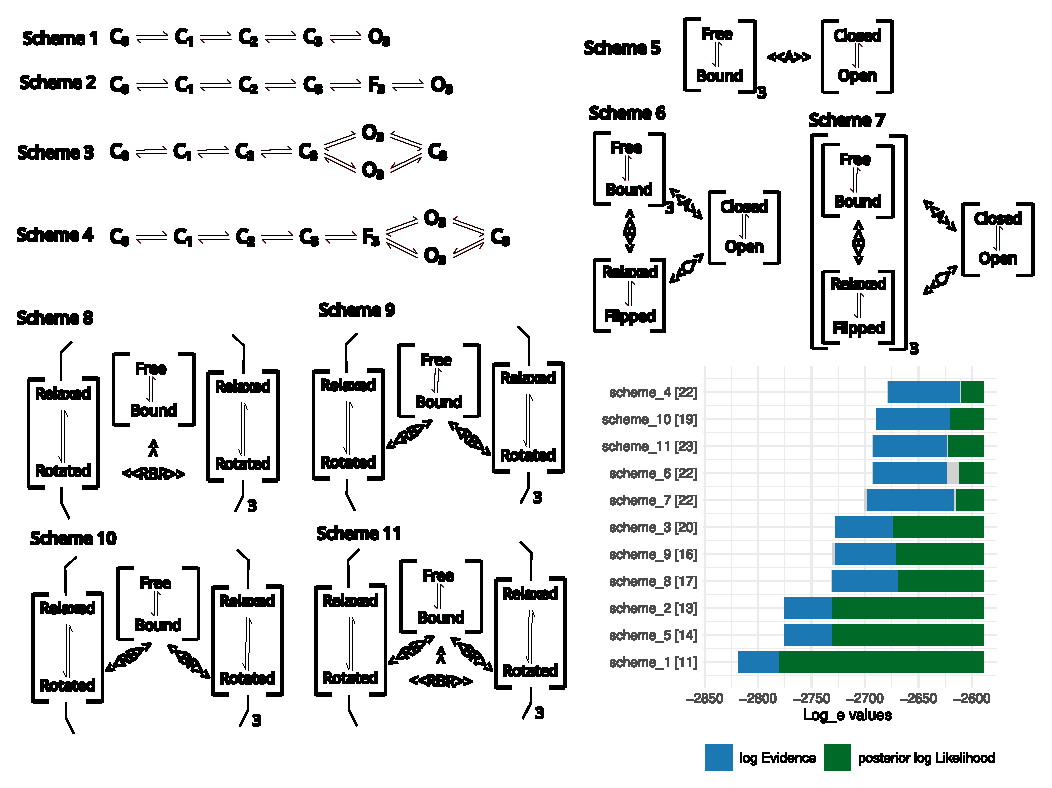
\includegraphics[width=1.0\textwidth]{Figure_1.eps}
\caption{Bayesian analysis of the tested kinetic schemes. For each tested kinetic scheme, the natural logarithm of the Evidence and posterior likelihood are indicated by the left end of the blue and green bars. Standard deviation of the samples are shown in light gray. Schemes are sorted according to their evidence, the highest at the top. Numbers in brackets next to the name of the schemes indicates the number of parameters. The length of the blue bar indicates the Kullback–Leibler divergence. }\label{fig_evidences}
\end{figure}



Highest Evidence was found for Scheme IV (\ref{fig_evidences}). That means that there still information in the kinetic responses that remains to be explained, Scheme IV does not explain it until we found a reasonable mechanistic counterpart. 
Then, all all the remaining schemes the one with the highest evidence is Scheme X. This tell us that sequential asymmetric gating is the most likely mechanism. There is strong evidence against a symmetrical gating (X vs IX) and there is evidence against a tertiary interaction with the other rotating subunit (X vs XI). All the gating mechanism is explained by an asymmetric binding induced conformational change. No inter-subunit interaction is detected by the models. 
Also, there is strong evidence that supports this sequential asymmetric gating model against a synchronous gating model (scheme VI). 
However, a more sophisticated (and computationally prohibitive) synchronous diffusive process (where rotation is a continuous and possibly contagious process) cannot be discarded, so there is still some chance for a synchronous model. 




\subsection{Posterior distribution of parameters of Scheme X: why is it bimodal}

\begin{figure}[h]
\centering
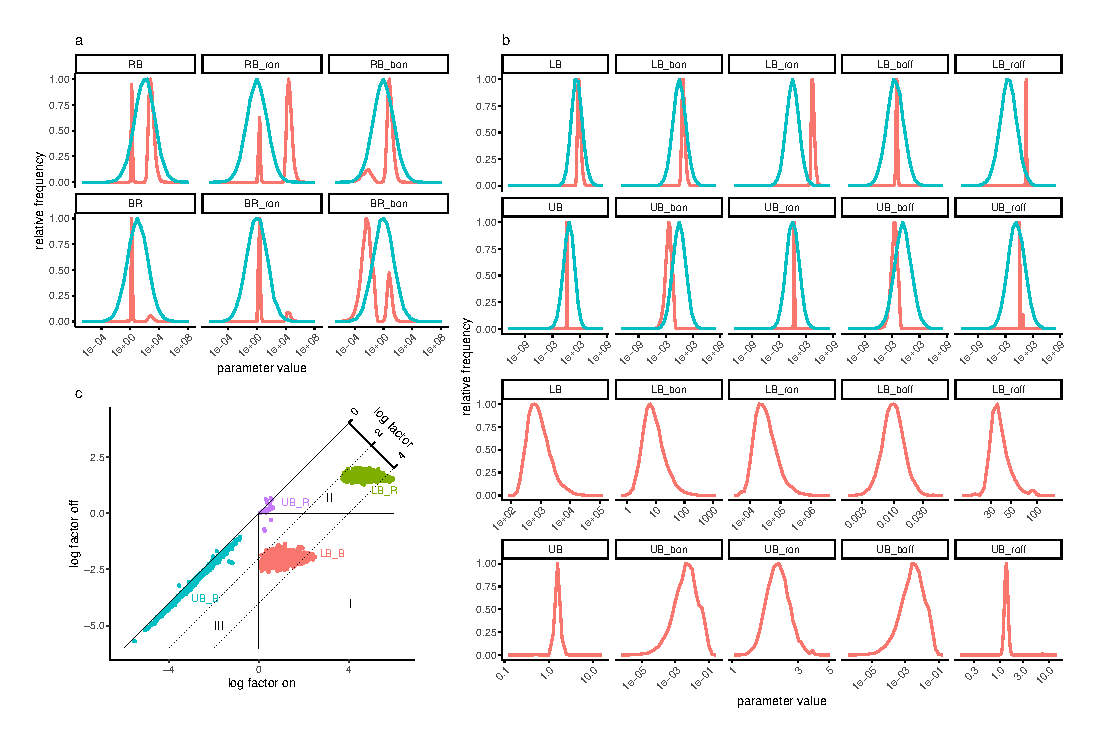
\includegraphics[width=1.0\textwidth]{Figure_2_ABC.eps}
\caption{Posterior distribution of allosteric parameters}
\label{fig_bimodal}
\end{figure}


Schemes cannot mathematically differentiate between interaction with the left subunit or the right subunit, there is no left-right information in the macrocurrents. Therefore it is not surprising that the posterior distribution of the allosteric parameters of scheme 10 are all bimodal. As a way to break such symmetry in the priors we arbitrarily set BR to be 10 times RB. However, as the prior standard deviation of the $log10$ of both parameters (and all the remaining ones) was set to be 2, there was enough exploration at low thermodynamic temperatures to jump from one minimum to the other, so both values appear, although at different frequencies. 
This bimodality can be removed by determining which is greater if RB or BR, and if the former if the case, swap all the remaining parameters. In this was unimodal distribution were recovered for all allosteric parameters. 

\subsection{Asymmetry in the allosteric coupling. analysis of parameters, rates and states}

Once we correct for the bimodality we find that whereas one interaction is considerable (100-10$^4$ times), the other is much smaller(0-2 times). So, upon binding, there is a strong allosteric interaction with one subunit and a weak interaction with the other. This second subunit will have strong interaction at the other binding site that it is forming. 
If we then look at the decomposition of the allosteric interaction we see the following.


\begin{figure}[h]
\centering
\includegraphics[width=1.0\textwidth]{Figure_3_definitive.pdf}
\caption{Posterior distribution of allosteric parameters}
\label{fig_bimodal}
\end{figure}


First, binding 




\subsection{One path for activating, another for deactivating}

\subsection{white and pink noise}

\subsection{partial conductance and opening with two ATPs}


For simultaneous rotation of all subunits, this would not make much of a difference, so scheme 6 works the same for intra subunit binding sites or inter-subunit binding sites. 









\section{Tables}\label{sec5}


\begin{table}[h]
\caption{Posterior distribution of Scheme X}\label{tab1}%
\begin{tabular}{c|c|c|c}
\hline
\hline
  parameters & median & CI\_hdi\_low & CI\_hdi\_hi \\ 
\hline
\hline
  \rowcolor[HTML]{efefef} 
  RB & 632.661 & 0.1441125 & 3.918861 10^{3} \\ 
  RB_{rot} & 2.454486 10^{4} & 1.260341 & 1.401152 10^{5} \\ 
  \rowcolor[HTML]{efefef} 
  RB_{bon} & 6.248909 & 1.933688 10^{-6} & 38.56124 \\ 
  BR & 1.612385 & 0.2657464 & 1.106451 10^{3} \\ 
  \rowcolor[HTML]{efefef} 
  BR_{rot} & 2.241492 & 1.077178 & 3.979711 10^{4} \\ 
  BR_{bon} & 6.986098 10^{-3} & 9.626552 10^{-7} & 11.16657 \\ 
\hline
\hline
\end{tabular}
\footnotetext{Source: This is an example of table footnote. This is an example of table footnote.}
\footnotetext[1]{Example for a first table footnote. This is an example of table footnote.}
\footnotetext[2]{Example for a second table footnote. This is an example of table footnote.}
\end{table}




\noindent

The input format for the above table is as follows:




\begin{table}[h]
\caption{Example of a lengthy table which is set to full textwidth}\label{tab2}
\begin{tabular*}{\textwidth}{@{\extracolsep\fill}lcccccc}
\toprule%
& \multicolumn{3}{@{}c@{}}{Element 1\footnotemark[1]} & \multicolumn{3}{@{}c@{}}{Element 2\footnotemark[2]} \\\cmidrule{2-4}\cmidrule{5-7}%
Project & Energy & $\sigma_{calc}$ & $\sigma_{expt}$ & Energy & $\sigma_{calc}$ & $\sigma_{expt}$ \\
\midrule
Element 3  & 990 A & 1168 & $1547\pm12$ & 780 A & 1166 & $1239\pm100$\\
Element 4  & 500 A & 961  & $922\pm10$  & 900 A & 1268 & $1092\pm40$\\
\botrule
\end{tabular*}
\footnotetext{Note: This is an example of table footnote. This is an example of table footnote this is an example of table footnote this is an example of~table footnote this is an example of table footnote.}
\footnotetext[1]{Example for a first table footnote.}
\footnotetext[2]{Example for a second table footnote.}
\end{table}

In case of double column layout, tables which do not fit in single column width should be set to full text width. For this, you need to use \verb+\begin{table*}+ \verb+...+ \verb+\end{table*}+ instead of \verb+\begin{table}+ \verb+...+ \verb+\end{table}+ environment. Lengthy tables which do not fit in textwidth should be set as rotated table. For this, you need to use \verb+\begin{sidewaystable}+ \verb+...+ \verb+\end{sidewaystable}+ instead of \verb+\begin{table*}+ \verb+...+ \verb+\end{table*}+ environment. This environment puts tables rotated to single column width. For tables rotated to double column width, use \verb+\begin{sidewaystable*}+ \verb+...+ \verb+\end{sidewaystable*}+.

\begin{sidewaystable}
\caption{Tables which are too long to fit, should be written using the ``sidewaystable'' environment as shown here}\label{tab3}
\begin{tabular*}{\textheight}{@{\extracolsep\fill}lcccccc}
\toprule%
& \multicolumn{3}{@{}c@{}}{Element 1\footnotemark[1]}& \multicolumn{3}{@{}c@{}}{Element\footnotemark[2]} \\\cmidrule{2-4}\cmidrule{5-7}%
Projectile & Energy	& $\sigma_{calc}$ & $\sigma_{expt}$ & Energy & $\sigma_{calc}$ & $\sigma_{expt}$ \\
\midrule
Element 3 & 990 A & 1168 & $1547\pm12$ & 780 A & 1166 & $1239\pm100$ \\
Element 4 & 500 A & 961  & $922\pm10$  & 900 A & 1268 & $1092\pm40$ \\
Element 5 & 990 A & 1168 & $1547\pm12$ & 780 A & 1166 & $1239\pm100$ \\
Element 6 & 500 A & 961  & $922\pm10$  & 900 A & 1268 & $1092\pm40$ \\
\botrule
\end{tabular*}
\footnotetext{Note: This is an example of table footnote this is an example of table footnote this is an example of table footnote this is an example of~table footnote this is an example of table footnote.}
\footnotetext[1]{This is an example of table footnote.}
\end{sidewaystable}

\section{Figures}\label{sec6}

As per the \LaTeX\ standards you need to use eps images for \LaTeX\ compilation and \verb+pdf/jpg/png+ images for \verb+PDFLaTeX+ compilation. This is one of the major difference between \LaTeX\ and \verb+PDFLaTeX+. Each image should be from a single input .eps/vector image file. Avoid using subfigures. The command for inserting images for \LaTeX\ and \verb+PDFLaTeX+ can be generalized. The package used to insert images in \verb+LaTeX/PDFLaTeX+ is the graphicx package. Figures can be inserted via the normal figure environment as shown in the below example:

%%=============================================%%
%% For presentation purpose, we have included  %%
%% \bigskip command. Please ignore this.       %%
%%=============================================%%
\bigskip
\begin{verbatim}
\begin{figure}[<placement-specifier>]
\centering
\includegraphics{<eps-file>}
\caption{<figure-caption>}\label{<figure-label>}
\end{figure}
\end{verbatim}
\bigskip
%%=============================================%%
%% For presentation purpose, we have included  %%
%% \bigskip command. Please ignore this.       %%
%%=============================================%%


\begin{figure}[h]
\centering
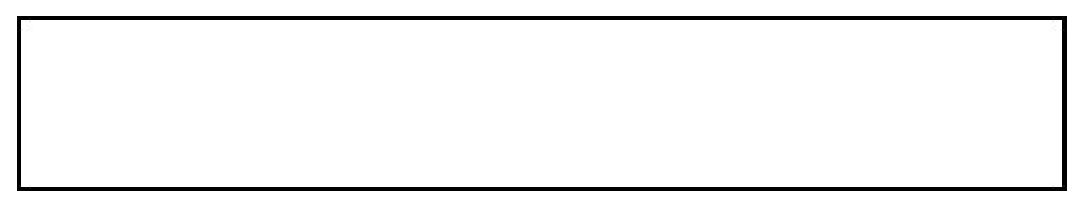
\includegraphics[width=0.9\textwidth]{fig.eps}
\caption{This is a widefig. This is an example of long caption this is an example of long caption  this is an example of long caption this is an example of long caption}\label{fig1}
\end{figure}

In case of double column layout, the above format puts figure captions/images to single column width. To get spanned images, we need to provide \verb+\begin{figure*}+ \verb+...+ \verb+\end{figure*}+.

For sample purpose, we have included the width of images in the optional argument of \verb+\includegraphics+ tag. Please ignore this. 

\section{Algorithms, Program codes and Listings}\label{sec7}

Packages \verb+algorithm+, \verb+algorithmicx+ and \verb+algpseudocode+ are used for setting algorithms in \LaTeX\ using the format:

%%=============================================%%
%% For presentation purpose, we have included  %%
%% \bigskip command. Please ignore this.       %%
%%=============================================%%
\bigskip
\begin{verbatim}
\begin{algorithm}
\caption{<alg-caption>}\label{<alg-label>}
\begin{algorithmic}[1]
. . .
\end{algorithmic}
\end{algorithm}
\end{verbatim}
\bigskip
%%=============================================%%
%% For presentation purpose, we have included  %%
%% \bigskip command. Please ignore this.       %%
%%=============================================%%

You may refer above listed package documentations for more details before setting \verb+algorithm+ environment. For program codes, the ``verbatim'' package is required and the command to be used is \verb+\begin{verbatim}+ \verb+...+ \verb+\end{verbatim}+. 

Similarly, for \verb+listings+, use the \verb+listings+ package. \verb+\begin{lstlisting}+ \verb+...+ \verb+\end{lstlisting}+ is used to set environments similar to \verb+verbatim+ environment. Refer to the \verb+lstlisting+ package documentation for more details.

A fast exponentiation procedure:

\lstset{texcl=true,basicstyle=\small\sf,commentstyle=\small\rm,mathescape=true,escapeinside={(*}{*)}}
\begin{lstlisting}
begin
  for $i:=1$ to $10$ step $1$ do
      expt($2,i$);  
      newline() od                (*\textrm{Comments will be set flush to the right margin}*)
where
proc expt($x,n$) $\equiv$
  $z:=1$;
  do if $n=0$ then exit fi;
     do if odd($n$) then exit fi;                 
        comment: (*\textrm{This is a comment statement;}*)
        $n:=n/2$; $x:=x*x$ od;
     { $n>0$ };
     $n:=n-1$; $z:=z*x$ od;
  print($z$). 
end
\end{lstlisting}

\begin{algorithm}
\caption{Calculate $y = x^n$}\label{algo1}
\begin{algorithmic}[1]
\Require $n \geq 0 \vee x \neq 0$
\Ensure $y = x^n$ 
\State $y \Leftarrow 1$
\If{$n < 0$}\label{algln2}
        \State $X \Leftarrow 1 / x$
        \State $N \Leftarrow -n$
\Else
        \State $X \Leftarrow x$
        \State $N \Leftarrow n$
\EndIf
\While{$N \neq 0$}
        \If{$N$ is even}
            \State $X \Leftarrow X \times X$
            \State $N \Leftarrow N / 2$
        \Else[$N$ is odd]
            \State $y \Leftarrow y \times X$
            \State $N \Leftarrow N - 1$
        \EndIf
\EndWhile
\end{algorithmic}
\end{algorithm}

%%=============================================%%
%% For presentation purpose, we have included  %%
%% \bigskip command. Please ignore this.       %%
%%=============================================%%
\bigskip
\begin{minipage}{\hsize}%
\lstset{frame=single,framexleftmargin=-1pt,framexrightmargin=-17pt,framesep=12pt,linewidth=0.98\textwidth,language=pascal}% Set your language (you can change the language for each code-block optionally)
%%% Start your code-block
\begin{lstlisting}
for i:=maxint to 0 do
begin
{ do nothing }
end;
Write('Case insensitive ');
Write('Pascal keywords.');
\end{lstlisting}
\end{minipage}


\section{Discussion}
\label{dis}


\section{Conclusion}
\label{con}


\backmatter

\bmhead{Supplementary information}

If your article has accompanying supplementary file/s please state so here. 

Authors reporting data from electrophoretic gels and blots should supply the full unprocessed scans for key as part of their Supplementary information. This may be requested by the editorial team/s if it is missing.

Please refer to Journal-level guidance for any specific requirements.

\bmhead{Acknowledgements}


Acknowledgements are not compulsory. Where included they should be brief. Grant or contribution numbers may be acknowledged.

Please refer to Journal-level guidance for any specific requirements.

\section*{Declarations}

Some journals require declarations to be submitted in a standardised format. Please check the Instructions for Authors of the journal to which you are submitting to see if you need to complete this section. If yes, your manuscript must contain the following sections under the heading `Declarations':

\begin{itemize}
\item Funding
\item Conflict of interest/Competing interests (check journal-specific guidelines for which heading to use)
\item Ethics approval and consent to participate
\item Consent for publication
\item Data availability 
\item Materials availability
\item Code availability 
\item Author contribution
\end{itemize}

\noindent
If any of the sections are not relevant to your manuscript, please include the heading and write `Not applicable' for that section. 

%%===================================================%%
%% For presentation purpose, we have included        %%
%% \bigskip command. Please ignore this.             %%
%%===================================================%%
\bigskip
\begin{flushleft}%
Editorial Policies for:

\bigskip\noindent
Springer journals and proceedings: \url{https://www.springer.com/gp/editorial-policies}

\bigskip\noindent
Nature Portfolio journals: \url{https://www.nature.com/nature-research/editorial-policies}

\bigskip\noindent
\textit{Scientific Reports}: \url{https://www.nature.com/srep/journal-policies/editorial-policies}

\bigskip\noindent
BMC journals: \url{https://www.biomedcentral.com/getpublished/editorial-policies}
\end{flushleft}

\begin{appendices}

\section{Section title of first appendix}\label{secA1}

An appendix contains supplementary information that is not an essential part of the text itself but which may be helpful in providing a more comprehensive understanding of the research problem or it is information that is too cumbersome to be included in the body of the paper.

%%=============================================%%
%% For submissions to Nature Portfolio Journals %%
%% please use the heading ``Extended Data''.   %%
%%=============================================%%

%%=============================================================%%
%% Sample for another appendix section			       %%
%%=============================================================%%

%% \section{Example of another appendix section}\label{secA2}%
%% Appendices may be used for helpful, supporting or essential material that would otherwise 
%% clutter, break up or be distracting to the text. Appendices can consist of sections, figures, 
%% tables and equations etc.

\end{appendices}

%%===========================================================================================%%
%% If you are submitting to one of the Nature Portfolio journals, using the eJP submission   %%
%% system, please include the references within the manuscript file itself. You may do this  %%
%% by copying the reference list from your .bbl file, paste it into the main manuscript .tex %%
%% file, and delete the associated \verb+\bibliography+ commands.                            %%
%%===========================================================================================%%

\bibliography{biblio}% common bib file
%% if required, the content of .bbl file can be included here once bbl is generated
%%\input sn-article.bbl


\end{document}
